\documentclass[sigplan,10pt]{acmart}

% review option: For printing line numbers:
%\documentclass[sigplan,10pt,review]{acmart} 

\settopmatter{printfolios=true,printccs=false,printacmref=false}
%printfolios=true, means print page numbers
%printccs=false, means don't show CCS categories
%printacmref=false, means don't show acm reference


\acmConference[Course paper, EDAN70]{Project in computer science}{Lund University}{Sweden}
\acmYear{\today}
\acmISBN{} % \acmISBN{978-x-xxxx-xxxx-x/YY/MM}
\acmDOI{} % \acmDOI{10.1145/nnnnnnn.nnnnnnn}
\startPage{1}

\setcopyright{none}

%% Bibliography style
\bibliographystyle{ACM-Reference-Format}
\usepackage{forest}
\usepackage{proof}
\newcommand{\NL}[0]{ \hfill\\\noindent }
\newcommand{\coloneqtwo}{\mathbin{:\hspace{-0.5ex}\textsf{-}}}
\begin{document}

%% Title information5
\title[Short Title]{Datalog Implementation in JastAdd (OUTLINE)}         %% [Short Title] is optional;
                                        %% when present, will be used in
                                        %% header instead of Full Title.
%\subtitle{Subtitle}                     %% \subtitle is optional


%% Author information
%% Each author should be introduced by \author, followed by
%% \affiliation, and \email.

\author{Hampus Balldin}
\affiliation{
  \institution{C13, Lund University, Sweden}            %% \institution is required
}
\email{dat12hba@student.lu.se}          %% \email is recommended


\begin{abstract}
Text of abstract \ldots.
\end{abstract}


\maketitle
\section{Introduction}
Datalog is a syntactically simple declarative language that allows the expression and evaluation of certain first-order logic propositions. From its' inception in the nineteen-eighties it received substantial interest from the academic community into the early nineteen-nineties\cite{Green:2013:DRQ:2688167.2688168}. The efforts primary drive were to enable knowledge based systems that allowed the generation of new facts based on rules stated using the logic programming paradigm. At the time, this had applications in both artificial intelligence as well as a complement to the traditional relational database querying systems such as SQL\cite{Ceri:1989:YAW:627272.627357}\cite{Bancilhon:1986:AIR:16894.16859}.

After a time of cooling interest, Datalog has emerged again as an attractive way to express complex inter-dependencies\cite{Green:2013:DRQ:2688167.2688168}. A notable example is from Program Analysis where frameworks such as Doop\cite{Smaragdakis:2010:UDF:2185923.2185939} make use of Datalog to derive e.g. call-graph and points-to information, both of which typically have mutually recursive dependencies in languages using dynamic dispatch. 

There are currently many Datalog implementations, some of which include Souffle\cite{Scholz:2016:FLP:2892208.2892226}, LogiQL\cite{Aref:2015:DIL:2723372.2742796}, Iris\cite{Bishop_iris-integrated}, and BDDBDDB\cite{Whaley:2005:UDB:2099708.2099719}. The implementations provide different evaluation methods and different extensions to the core Datalog language. This paper describes a common front-end that allows for source-to-source compilation. A common front-end enables a convenient way to compare the performance and expressive power of different Datalog implementations. An additional goal is to provide a library that can be used to implement and evaluate new inference schemes.

JastAdd \cite{Ekman:2007:JEJ:1297105.1297029} is a meta-compilation system that enables the expression of arbitrary graphs on top of an abstract syntax tree (AST). Information is propagated through the AST using so called Reference Attribute Grammars. JastAdd also supports aspects which allow the weaving of methods and class fields from different source locations into a single generated class. This enables easy extension of the generated AST classes with additional properties. In particular, it nicely permits the incremental addition of support for source-to-source compilation to different Datalog implementations. 

\subsection{Core Language}
There are many flavors of the Datalog language but they all build on a common core. 

%A \textit{program} $P$ consists of a set of \textit{Horn clauses} $H_1, \ldots H_n$. A horn clause has a \textit{head} and a \textit{body}. The head is a single \textit{atom} and the body is a sequence of atoms. A atom is identified by a \textit{predicate symbol} and a sequence of g\textit{terms}. An example of a propositional rule (without terms) is shown below:
\begin{align*}
A :- \;B_1, B_2, \ldots B_m
\end{align*}
\noindent
Above we have a single horn clause (hereafter called a \textit{rule}). It has head $A$ and body $B_1, B_2, \ldots B_m$. The intuitive meaning of the above rule is that if the conjunction of all the atoms in the body are true then we conclude $A$.

Datalog deals not only with propositional rules, but allows a restricted range of first-order propositions where each atom is associated with a sequence of terms. A term is either \textit{variable} or \textit{constant}. An atom that contain only constant terms is called a \textit{ground atom}. We further partition the predicates into extensional (EDB) and intensional (IDB). The EDB's are all predicates that are taken as input from an external database. The IDB's are the predicates that are not EDB and are intensionally defined through rules. The EDB's introduce \textit{facts}, i.e. ground atoms. One may additionally introduce facts by declaring a rule with a ground atom head that has an empty body. 

\begin{itemize}
\item The set of all constants in all facts is called the \textit{domain} and is denoted $\Omega$.
\item The set of all facts is called the \textit{active database instance} and is denoted $I$.
\end{itemize}
 
There are three main semantic interpretations of Datalog: model-, fixpoint-, and proof-theoretic semantics. \cite{Green:2013:DRQ:2688167.2688168}. A brief overview is given below.

\paragraph{Model-theoretic Semantics}\NL
A \textit{model} of a Datalog program $P$ is a consistent (satisfying all rules of $P$) extension of the initial EDB facts. Each rule is interpreted as a universally quantified rule. For example, below is given a rule and its' corresponding semantic interpretation. In the example $B(c_1, "C")$ is written as $(c_1, "C") \in B$ to emphasize the practical correspondence between predicates and relations.
\begin{align*}
A(x, y, "C") :- \;B_1(x, "C"), B_2("C", y), B_3(x, y)
\end{align*}
\begin{align*}
\infer{(c_1, c_2, "C") \in A}{%
	\forall c_1 \in \Omega.\;\forall c_2 \in \Omega. \;\; (c_1, "C") \in B_1, ("C", c_2) \in B_2, (c_1,c_2) \in B_3
}
\end{align*}
An inference algorithm attempts to find the \textit{minimal model}, i.e. a model $m$ of $P$ such that for any other model $m'$ of $P$, all facts of $m$ are in $m'$. In practice this means that an inference algorithm should only add a fact if it is required by the semantics of a rule (even if adding the fact may lead to an extended model of $P$). 

\paragraph{Fixpoint-theoretic Semantics}\NL
Begin with the set of all facts in the active database instance $I^0$. The set of new facts that can be derived (under model-theoretic semantics) using the rules of a program $P$ and the existing facts in $I^i$ is denoted $\Delta_i$. We get the following inductive definition of $I$:
\begin{align*}
&I^0 = \{ \text{EDB Facts in } P \}\\
&I^{i + 1} = I^i \cup \Delta_i 
\end{align*}
It can be shown(CITE) that the minimal model is computed as $I^{n}$ for $n$ such that $I^{n}$ = $I^{n + 1}$. Since $I^i \subseteq I^{i + 1}$ (monotonically increasing) and with the practical assumption of a finite domain, the fix-point algorithm is guaranteed to terminate.

\paragraph{Proof-theoretic Semantics}\NL
Consider a ground atom $A(C_1, \ldots, C_n)$. A query for the ground atom asks for a proof that $A(C_1, \ldots, C_n)$ is in the minimal model of a program $P$. A proof can be visualized as an \textit{and-or tree} $T$. $T$ has the proposition (ground atom) to prove as the root. At an OR-node, all possible rules are tested. If any of them succeed then the proposition has been proven. At an AND-node, all the child propositions need to be proven for the node to become true. An example is shown in figure \ref{figure:andOrTree}.
\begin{align*}
r_1: A :- \;B, C\\
r_2: A :- \;B, D
\end{align*}
\begin{figure}[ht!]
  \centering

\begin{forest}
for tree={circle, draw, l sep=1pt}
[A,blue 
	[$\lor$  
		[$\land$, edge label={node[midway,left] {$r_1$}}
			[B] 
			[C] 
		]
		[$\land$, edge label={node[midway,right] {$r_2$}}
			[B]
			[D]
		]
	]
]
\end{forest}
\caption{An and-or tree for rules $r_1: A :- \;B, C$, $r_2: A :- \;B, D$}
\label{figure:andOrTree}
\end{figure}
\noindent
When traversing the tree the model is updated with new facts that are needed to prove the root proposition. Those facts then become part of the extended model. 

\subsection{Security Features and Time Complexity}
Above a fact was stated to be a ground atom that is true in a given model. An axiomatic fact can be declared as a rule with no body: $A(t_1, \ldots, t_n)$. Datalog disallows axiomatic facts that contain variables. This is implied by the following more general rule: all variables occurring in the head of a rule must also occur in the body of the rule. This is called the \textit{range restriction property} \cite{Green:2013:DRQ:2688167.2688168}.

\subsection{Query Evaluation}



% Expression Problem
% (Knuth attribute Grammars)
% Parser / Lexer
% (How much is interesting to write here?)
\section{Core Language Implementation}
\newcommand{\sigmatwo}{\overline{\sigma}}
The current query evaluation mechanism for \datalogM is a bottom-up naive\cite{Green:2013:DRQ:2688167.2688168} evaluation. It is based on the fixpoint-theoretic semantics, deriving tuples from rules until no new tuples may be derived. The rule evaluation is performed using relational algebra (see e.g. \cite{Abiteboul:1995:FDL:551350}) and a thorough description is given in Appendix A.

\subsection{Mutual Dependencies and Predicate Ordering}
With multiple rules and potentially many mutual dependencies between the predicates, there is a need to find an order in which to apply the rules. Indeed, for mutually dependent predicates, all rules which may derive new facts for those predicates need to be iterated together. \textit{Stratification}\cite{Green:2013:DRQ:2688167.2688168} is the process of clustering the predicates that need to be computed together into so called \textit{strata} as well as to find an optimal order between the strata. The iterative fix-point algorithm is then run over each \textit{stratum} following the computed order. The process is formalized below.

A predicate $P_i$ \textit{directly depends} on predicate $P_j$ iff there exists a rule for which $P_i$ is in the head and $P_j$ is in the body. Let $Dep(P_i)$ be the set of predicates which $P_i$ directly depends on. The dependency graph $G_{DEP}$ has the set of predicate symbols as vertices and there is an edge from $P_i$ to $P_j$ iff $P_j \in DEP(P_i)$. A strongly connected component in $G_{DEP}$ then contains the predicates which are mutually recursive. Such a connected component can be found e.g. using Tarjan's algorithm \cite{Tarjan72depthfirst} and is called a stratum. By merging the vertices of $G_{DEP}$ into such strata we get a graph $G_{STRAT}$ with vertices being the strata of $G_{DEP}$ and edges the collapsed multi-edges from $G_{DEP}$. By construction there exists a total order on $G_{STRAT}$ with $S_1 < S_2$ iff $(S_1, S_2) \in Edge(G_{STRAT})$. The desired order is found by a reverse post-order search of $G_{STRAT}$.
\begin{figure*}[!hbt]
	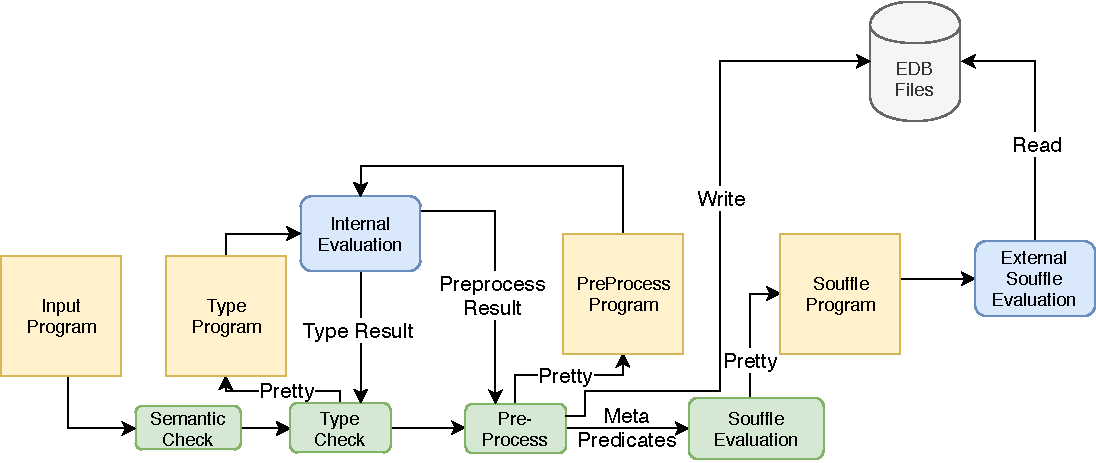
\includegraphics[scale=0.7]{img/souffleEval.pdf}
	\caption{Souffle Printing Pipeline. \textbf{Yellow}: A Datalog Program. \textbf{Blue}: An evaluation mechanism. \textbf{Green}: A compiler stage. }
	\label{figure:soufflePipeline}
\end{figure*}
\subsection{Cross Compilation}
In addition to internal evaluation, $Datalog^M$ supports cross-compilation, or pretty-printing, to Souffle\cite{SouffleHome}. The compilation pipeline is shown in figure \ref{figure:soufflePipeline}. First, a number of semantic checks are performed. For example, the semantic check ensures that all variables used in the head of a rule also occures in the body of the rule (the range restriction property\cite{Ceri:1989:YAW:627272.627357}). In the next stage, the program is type checked (type-checking is described in more detail in the following section). As was mentioned in the introduction (and will be explained in the next section), \datalogM supports meta-predicates. Souffle however has no such support so naturally it does not recognize the meta-semantics. To this end, a separate pre-process Datalog program is generated to evaluate all meta-predicates and subsequently output them as EDB files. Finally, the program is pretty-printed to a Souffle program $P_{Souffle}$. $P_{Souffle}$ declares the meta-predicates and loads them from the EDB files; the meta-predicates can then be used as ordinary predicates within the Souffle environment.
\section{Language Extensions}
\subsection{Type System}
\subsection{Negation}
\subsection{Object Creation}
\subsection{Built-in Predicates}
\section{Evaluation}

\textit{I want to use the following evaluation criteria}
\begin{itemize}
\item Front-end extensibility
\item Front-end source-to-source coverage
\item Back-end implementations performance evaluation
\end{itemize}

\section{Related work}
\subsection{LogicBlox}
\subsection{Iris}
\subsection{Souffle}
\subsection{BDDBDDB}
\section{Conclusion}
%% Acknowledgments
\begin{acks}
Text of acknowledgments \ldots.
\end{acks}


%% Bibliography
\bibliography{bibl}



\end{document}
